\documentclass[twoside]{article}

%\usepackage{aistats2022}
% If your paper is accepted, change the options for the package
% aistats2022 as follows:
%

\usepackage{aistats2022}
\usepackage{amsthm}
\usepackage{amsfonts}
\usepackage{amsmath}
\usepackage{amssymb,bbm}
\usepackage{algorithm,algorithmic}
\usepackage{natbib}
\usepackage{graphicx}

%
% This option will print headings for the title of your paper and
% headings for the authors names, plus a copyright note at the end of
% the first column of the first page.

% If you set papersize explicitly, activate the following three lines:
\special{papersize = 8.5in, 11in}
\setlength{\pdfpageheight}{11in}
\setlength{\pdfpagewidth}{8.5in}
% If you use natbib package, activate the following three lines:
%\usepackage[round]{natbib}
%\renewcommand{\bibname}{References}
%\renewcommand{\bibsection}{\subsubsection*{\bibname}}

% If you use BibTeX in apalike style, activate the following line:
%\bibliographystyle{apalike}
\theoremstyle{plain}
\newtheorem{thm}{Theorem}
\newtheorem*{thm*}{Theorem}
\newtheorem{lem}[thm]{Lemma}
\newtheorem{prop}[thm]{Proposition}
\newtheorem{cor}[thm]{Corollary}
\newtheorem{conj}[thm]{Conjecture}
\newcommand{\y}{\mathbf y}
\newcommand{\C}{\mathbf C}
\newcommand{\T}{\mathbf T}
\newcommand{\calC} {\mathcal{C}}
\newcommand{\bfP} {\mathbf{P}}
\newcommand{\kl}{\mathbf {KL}}
\newcommand{\kll}{\mathcal {KL}}
\newcommand{\OTmp}[1]{\hat{\mathbf{P}}_{#1}}
\newcommand{\prox}{\operatorname{prox}}
\newcommand{\proj}{\operatorname{Proj}}
\newcommand{\diag}{\operatorname{diag}}
\newcommand{\argmin}{\operatorname{argmin}}
\newcommand{\tranT}{\mathsf T}
\newcommand{\X}{\mathbf{X}}
\newcommand{\x}{\mathbf{x}}
\newcommand{\R}{\mathbbm{R}}
\newcommand{\one}{\mathbbm{1}}
\newcommand{\ma}{\mathbf{a}}
\newcommand{\mb}{\mathbf{b}}
\newcommand{\vc}{\mathbf c}
\newcommand{\vt}{\mathbf t}


\begin{document}

% If your paper is accepted and the title of your paper is very long,
% the style will print as headings an error message. Use the following
% command to supply a shorter title of your paper so that it can be
% used as headings.
%
%\runningtitle{I use this title instead because the last one was very long}

% If your paper is accepted and the number of authors is large, the
% style will print as headings an error message. Use the following
% command to supply a shorter version of the authors names so that
% they can be used as headings (for example, use only the surnames)
%
%\runningauthor{Surname 1, Surname 2, Surname 3, ...., Surname n}

\twocolumn[

\aistatstitle{Dynamic Screening Method on the Unbalanced Optimal Transport Problem}

\aistatsauthor{ Xun Su \And Author 2 \And  Author 3 }

\aistatsaddress{ Waseda University \And  Institution 2 \And Institution 3 } ]

\begin{abstract}
This paper promote a dynamic screening framework for Unbalanced Optimal Transport (UOT) problem. Recently, researchers connected the UOT problem with Lasso problem, which encourage us to apply the common speeding up method screening on the UOT problem. We demonstrate the effectiveness of the screening method and propose a better improvement to it based on the unique structure of the UOT problem. We constructed several experiments on the problem and they indicate that... 

\end{abstract}


Optimal Transfer (OT) has a long history in mathematics and has recently become prevalent due to its important role in the machine learning community for measuring distances between histograms. It has outperformed traditional methods in many different areas such as domain adaptation \citep{7586038}, generative models \citep{arjovsky2017wasserstein},, graph machine learning \citep{NEURIPS2019_fdd5b16f} and natural language processing. \citep{084adf2f555549c493e0331a00e4ecad} Its popularity is attributed to the introduction of Sinkhorn's algorithm for the entropy optimal transmission problem, \citep{NIPS2013_af21d0c9} which improves the computational speed of the OT problem from $\Theta (n^3)$ of Simplex's method to $\Theta (n^2)$. In order to extend the optimal transmission problem, which can only handle balanced samples, to a wider range of unbalanced samples. The unbalanced optimal transport (UOT) is proposed by modifying the restriction term to a penalty function term. UOT has been used in several applications like computational biology \citep{SCHIEBINGER2019928} , machine learning \citep{DBLP:conf/aistats/JanatiCG19} and deep learning \citep{DBLP:conf/iclr/YangU19}. 

The UOT problem is a regularized version of Kantorovich formulation which replaced the equality constraints with penalty functions on the marginal distributions with a divergence. Many different divergences have been taken into consideration for UOT problems like $KL$ divergence, $l_1$ norm, and $L_2$ norm. When it comes to the solving method, $KL$ penalty with the entropy form can be solved by the Sinkhorn algorithm. It provides the UOT computation with scalability and differentiability but suffers from a larger error of $KL$ divergence and lack of sparsity in solution compared with other regularizers \citep{DBLP:conf/aistats/BlondelSR18}. However, $L_2$ norm could bring a sparse solution, which attracted the attention of researchers and many new algorithms are developed for it. \citep{NEURIPS2021_c3c617a9}, \citep{https://doi.org/10.48550/arxiv.2202.03618} At the same time, The link between the UOT problem with many other well-known problems such as non-negative matrix decomposition and Lasso problem has been discovered, which encourages researchers to improve it by using the rich results in these fields.

Screening is a well-known technique proposed by \citep{ghaoui2010safe} in the field of lasso problems, where the $L_1$ regularizer leads to a sparse solution for the problem. It can pre-select solutions that must be zero theoretically and freeze them before computation. The solutions to many large-scale optimization problems are sparse, and a large amount of computation is wasted on updating the zero elements. With the Safe Screening method, we can identify and freeze the elements that are zero with linear complexity computation before starting the algorithm, thus saving optimization time. the Screening method get attention in recent years and has been improved a lot, New methods such as Dynamic Screening \citep{7128732}, Gap screening method \citep{JMLR:v18:16-577} and Dynamic Sasvi \citep{NEURIPS2021_7b5b23f4}  

The OT and UOT problems produce extremely sparse solutions due to the effectiveness of their optimal transport cost, which is a similar operator to the Lasso problem. We believe that it indicates the potential effectiveness of applying screening technical in the Lasso problem to the UOT problem. Furthermore, Different from the Lasso problem which has a dense constraints matrix, the UOT problem's constraint matrix is extremely sparse and has a unique transport matrix structure, which would benefit the design of screening and the outcome.


\textbf{Contribution}: 
\begin{itemize}
\item We systematically provide the newest framework for the Screening method on the UOT problem. Considering the sparse and specific structure of the UOT problem, we design a new projection method for UOT screening, which hugely improves the screening performance over the general Lasso method.
\item We propose a two-plane screening method for UOT problems, which benefits from UOT's sparse constraints and outperforms the ordinary methods adding only a negligible amount of computation
\end{itemize}




\section{Background}
\subsection{Optimal Transport and Unbalanced Optimal Transport}
Given two histograms $\alpha \in \mathbbm{R}^{m}, \beta \in \mathbbm{R}^{n},$ For a cost matrix $C \in \mathbbm{R}^{m \times n}$, Optimal transport problem is trying to get a corresponding transport matrix $T \in \mathbbm{R}^{m \times n}$ that minimize the whole transport cost, which could be formulated as:
$$
\begin{aligned}
W(\alpha,\beta) := \min_{ \mathbf{T} \in \mathbb{R}_{+}^{n \times n},\mathbf{T} \mathbbm{1} = \alpha, \mathbf{T}^{T}\mathbbm{1} = \beta} \langle \C, \mathbf{T} \rangle 
\end{aligned}
$$

We can write it into a vector type, set $c,t \in \mathbbm{R}^{mn}$:
$$
\begin{aligned}
W(\alpha,\beta) := \min_{t \in \mathbb{R}_{+}^{n^2}, \mathbf{N}t = \alpha, \mathbf{M}t = \beta} c^{\tranT}t 
\end{aligned}
$$

$\mathbf{N} \in \mathbbm{R}^{m \times mn}, \mathbf{N} \in \mathbbm{R}^{n \times mn}$ are two matrix consisted with 0 and 1, listed in Appendix.A. We define $y = [\alpha, \beta]^{\tranT}$, the UOT problem add a penalty function for the historgrams: 
\begin{equation}
\label{eq:uot}
W(\alpha,\beta) := \min_{t \in \mathbb{R}_{+}^{mn}} c^{\tranT}t + D_h(\mathbf{X}t,y)
\end{equation}
$D_h$ is the Bregman divergence and $h$ is the norm, $\X = [\mathbf{M}^{\tranT} \mathbf{N}^{\tranT}]^{\tranT}$.

\subsection{Relationship with Lasso}
Lasso-like problem has a general formula as:
$$
\begin{aligned}
f(t) = g(t) + D_h(\X t,b), t\in \mathbbm{R}^{mn}
\end{aligned}
$$
When $g(t) = \lambda \|t\|$ and $D_h(\X t,b) = \|\X t-b\|_2^2$, this is the Euclid regression Lasso problem


\subsection{Dynamic Screening Framework}

We follow \cite{NEURIPS2021_7b5b23f4}'s framework to introduce about the whole dynamic screening technique for Lasso-like problem:
\begin{equation}
\label{eq:lassolike}
f(t) = g(t) + d(\X t)
\end{equation}

By Frenchel-Rockafellar Duality, we get the dual problem
\begin{thm}
 (Frenchel-Rockafellar Duality) If $d$ and $g$ are proper convex functions on $\mathbbm{R}^{m+n}$ and $\mathbbm{R}^{mn}$. Then we have the following:
 $$
\begin{aligned}
\min_t  g(t) + d(Xt) = \max_{\theta} -d^*(-\theta)-g^*(X^{\tranT}\theta)
\end{aligned}
$$
\end{thm}

Because the primal function $d$ is always convex, the dual function $d^*$ is concave. Assuming $d^*$ is an L-strongly concave problem. we design an area for any $\tilde{\theta}$ by the strongly concave property:

\begin{thm}\label{circle}
(L-strongly concave) Considering problem \ref{eq:lassolike}, if $d$ and $g$ are both convex, for $\forall \theta \in{R^{m+n}}$, we have the following:  
$$
\begin{aligned}
\theta \in \{\frac{L}{2}\|\theta-\tilde{\theta}\|_2^2+d^*(-\tilde{\theta}) \leq d^*(-\theta)\}
\end{aligned}
$$
\end{thm}
We know that the optimal solution for the dual problem $\hat{\theta}$ satisfied the inequality, so the set is not empty.
We can get the dual form of Lasso-like problem for some specific functions: 
\begin{lem}
For $d(\X t) = \frac{1}{2}\|\X t-y\|_2^2$, the dual Lasso problem has the following form:
$$
\begin{aligned}
d^*(-\theta) = \frac{1}{2}\|\theta\|_2^2-y^{\tranT}\theta
\end{aligned}
$$

$$
g^*(X^{\tranT}\theta) = \left\{
\begin{aligned}
0 \quad&\quad ( \forall t \quad\theta^{\tranT}Xt - g(t) \leq 0 )\\
\infty \quad&( \exists t \quad\theta^{\tranT}Xt - g(t) \leq 0 )
\end{aligned}
\right.
$$
\end{lem}






















\section{Dynamic Screening and UOT problem}
\subsection{Screening for UOT}

For UOT problem \ref{eq:uot}, we could get its dual form. 
\begin{lem}(Dual form of UOT problem)
\begin{equation}
\begin{split}
-d^*(-\theta) - g^*(X^{\tranT}\theta)& = -\frac{1}{2}\|\theta\|_2^2-y^{\tranT}\theta \\
 \mathbf{s.t.} \quad \forall i \quad x_i^{\tranT}\theta -\lambda c_i &\leq 0
 \end{split}
 \label{eq:uotdual}
\end{equation}
\end{lem}
The equation indicate a dual feasible area constructed by many dual constraints, the optimal solution is inside the constraints.\\
From the KKT condition, we can make sure that, for the optimal primal solution $\hat{t}$:
\begin{thm} (Screening) For the dual optimal solution $\hat{\theta}$, we have the following relationship:
 \begin{equation}
\begin{split}
x_i^{\tranT}\hat{\theta} -\lambda c_i  \left\{
\begin{aligned}
< 0 \quad& \Rightarrow \hat{t}_i = 0\\
= 0 \quad& \Rightarrow \hat{t}_i \geq 0
\end{aligned}
\right.
 \end{split}
 \label{eq:screening}
\end{equation}
\end{thm}

As we do not know the information of $\hat{t}$ directly, we can construct an area $\mathcal{R}^{S}$ containing the $\hat{t}$, if

 \begin{equation}
\max_{t \in \mathcal{R}^S} x_i^{\tranT}\theta -\lambda c_i  < 0
\end{equation}
then we have:
 \begin{equation}
 x_i^{\tranT}\hat{\theta} -\lambda c_i  < 0
\end{equation}
which means the corresponding $\hat{t}_i = 0$, and can be screening out.

Now we start to construct the area containing $\hat{\theta}$, from \ref{circle} we know that the $\hat{\theta}$ is inside the intersection of the area of \ref{circle} and the dual feasible area. However, the multilinear constraints make it hard to compute the maximum for the problem, We design a relaxation method. which divide the constrains into two parts, then we are maximizing on the intersection of two hyperplane and a hyper-ball. 

\begin{thm}\label{area}
$$
\mathcal{R}^S = \{ nihao \}
$$
\end{thm}
the computational process is in Appendix.A

\subsection{Screening Algorithms}

 \begin{algorithm}
 \caption{UOT Dynamic Screening Algorithm}
 \begin{algorithmic}[1]
 \renewcommand{\algorithmicrequire}{\textbf{Input:}}
 \renewcommand{\algorithmicensure}{\textbf{Output:}}
 \REQUIRE $t_0, S \in R^{n\times m}, S_{ij}=1$
 \ENSURE  $S$
  \STATE \text{Choose a solver for the problem.}
  \FOR {$t = 0 \text{ to } K$}
  \STATE $\text{Projection } \tilde{\theta} = \operatorname{Proj}(t_k)$ 
  \IF {($i \ne 0$)}
  \STATE $\textbf{break}$
  \ENDIF
    \STATE $\mathcal{R} \Leftarrow \mathcal{R}^S{(\tilde{\theta},t_k)}$
    \STATE $S \Leftarrow {S_{ij} = 0 \text{ if } \max_{\theta \in \mathcal{R}^S} {x_{k(i,j)}}^{\tranT}\theta <\lambda c_{k(i,j)} }$
    \FOR {$a  \in {A_{ij}\|A_{ij}=0}$}
    \STATE $t_k(i,j) \Leftarrow 0$
    \ENDFOR
    \STATE $t_{k+1} = \operatorname{update}(t_k)$
  \ENDFOR
  
 \RETURN $t_{K+1}, S $ 
 \end{algorithmic} 
 \end{algorithm}

screening method is irrelevent to the optimization solver you choose. We gave the specific algorithm for $L_2$ UOT problem to show the whole optimization process.\\
An important part is that we use the primal solution to compute a dual solution, which might not inside the dual feasible area, a projection method is necessary. We promote a new projection method for the UOT problem for its sparse matrix structure.

\begin{thm}\label{proj}
$$
\tilde{\theta} = 1
$$
\end{thm}












































\section{Experiments}
In this section, we show the efficacy of the proposed methods using a toy Gaussian model and the MNIST dataset.
\subsection{Projection Method}
In order to prove the rightness of our projection method compared with the traditional projection method in lasso problem, we compared the screening ratio with random generated Gaussian measures by two projection method. We set the $\lambda = \frac{\|\mathbf{X}^{\tranT}y\|}{100}$ and test for 10 different pairs.We choose FISTA for solving $L_2$ penalized UOT problem. 
	\begin{figure}[htbp]
	\begin{center}	
	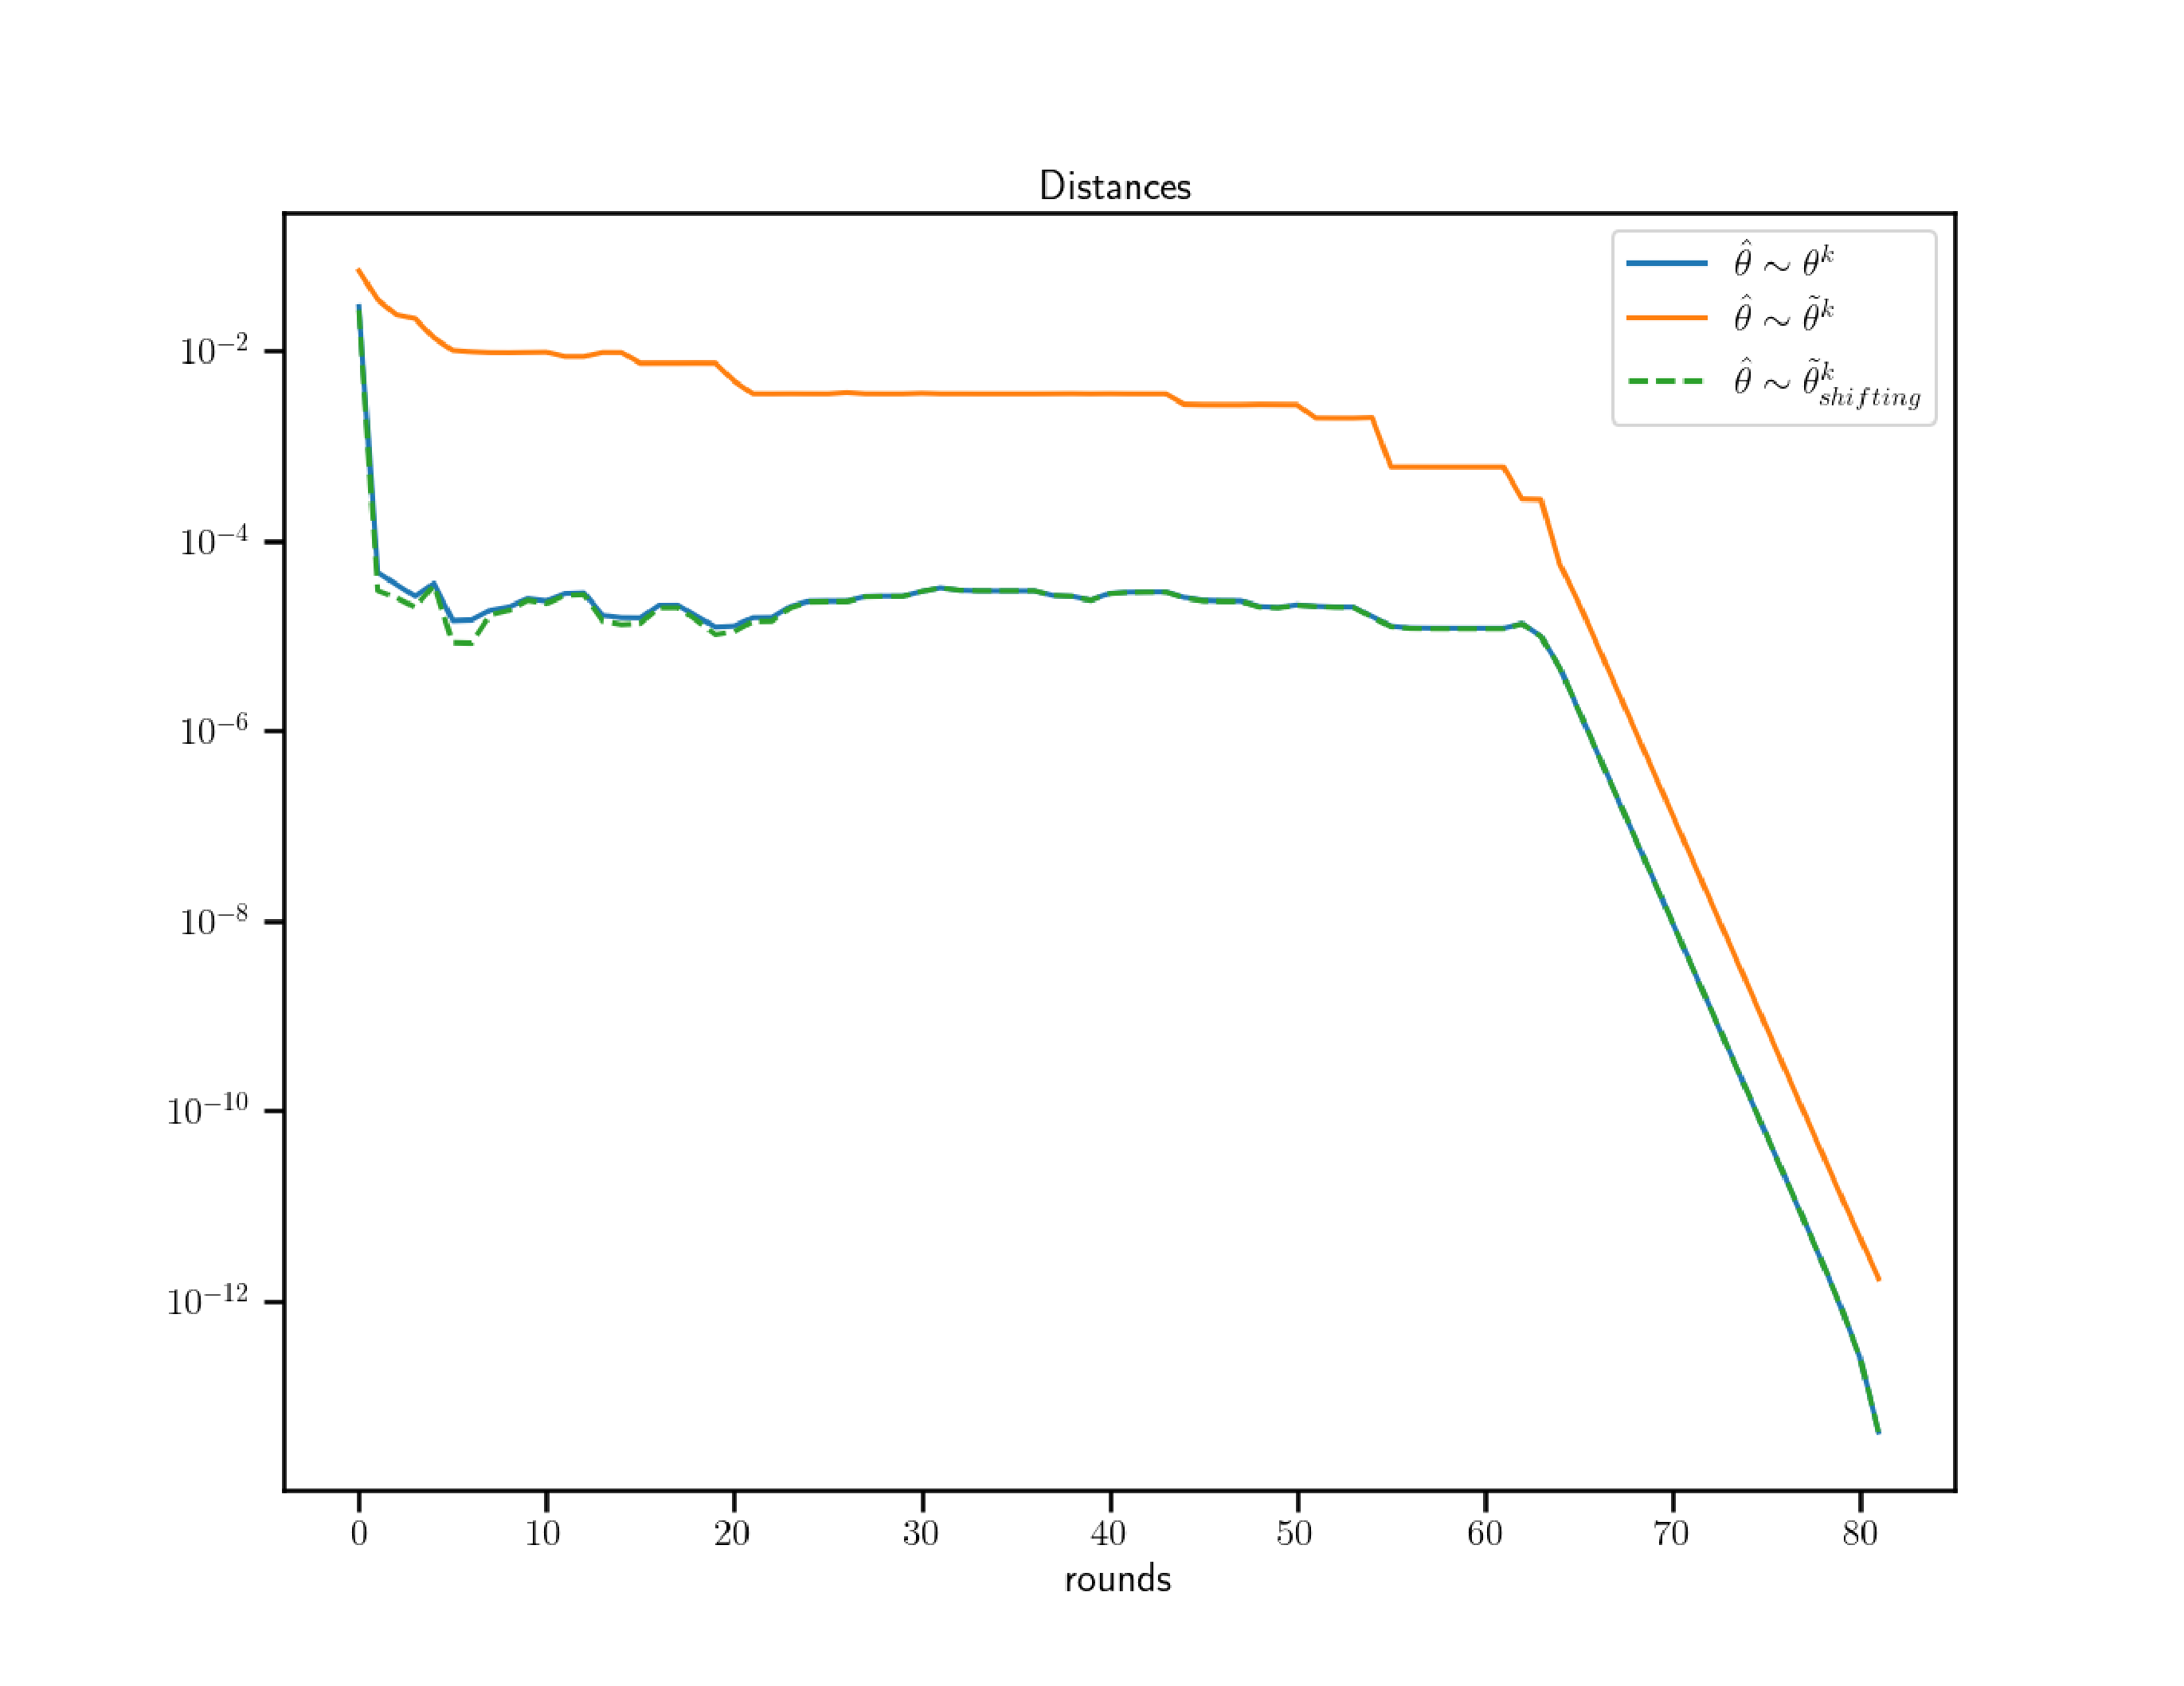
\includegraphics[width=0.4\hsize]{pic/projdis}
	\caption{Distance of different projection method}
	\end{center}	
	\end{figure}
	\begin{figure}[htbp]
	\begin{center}	
	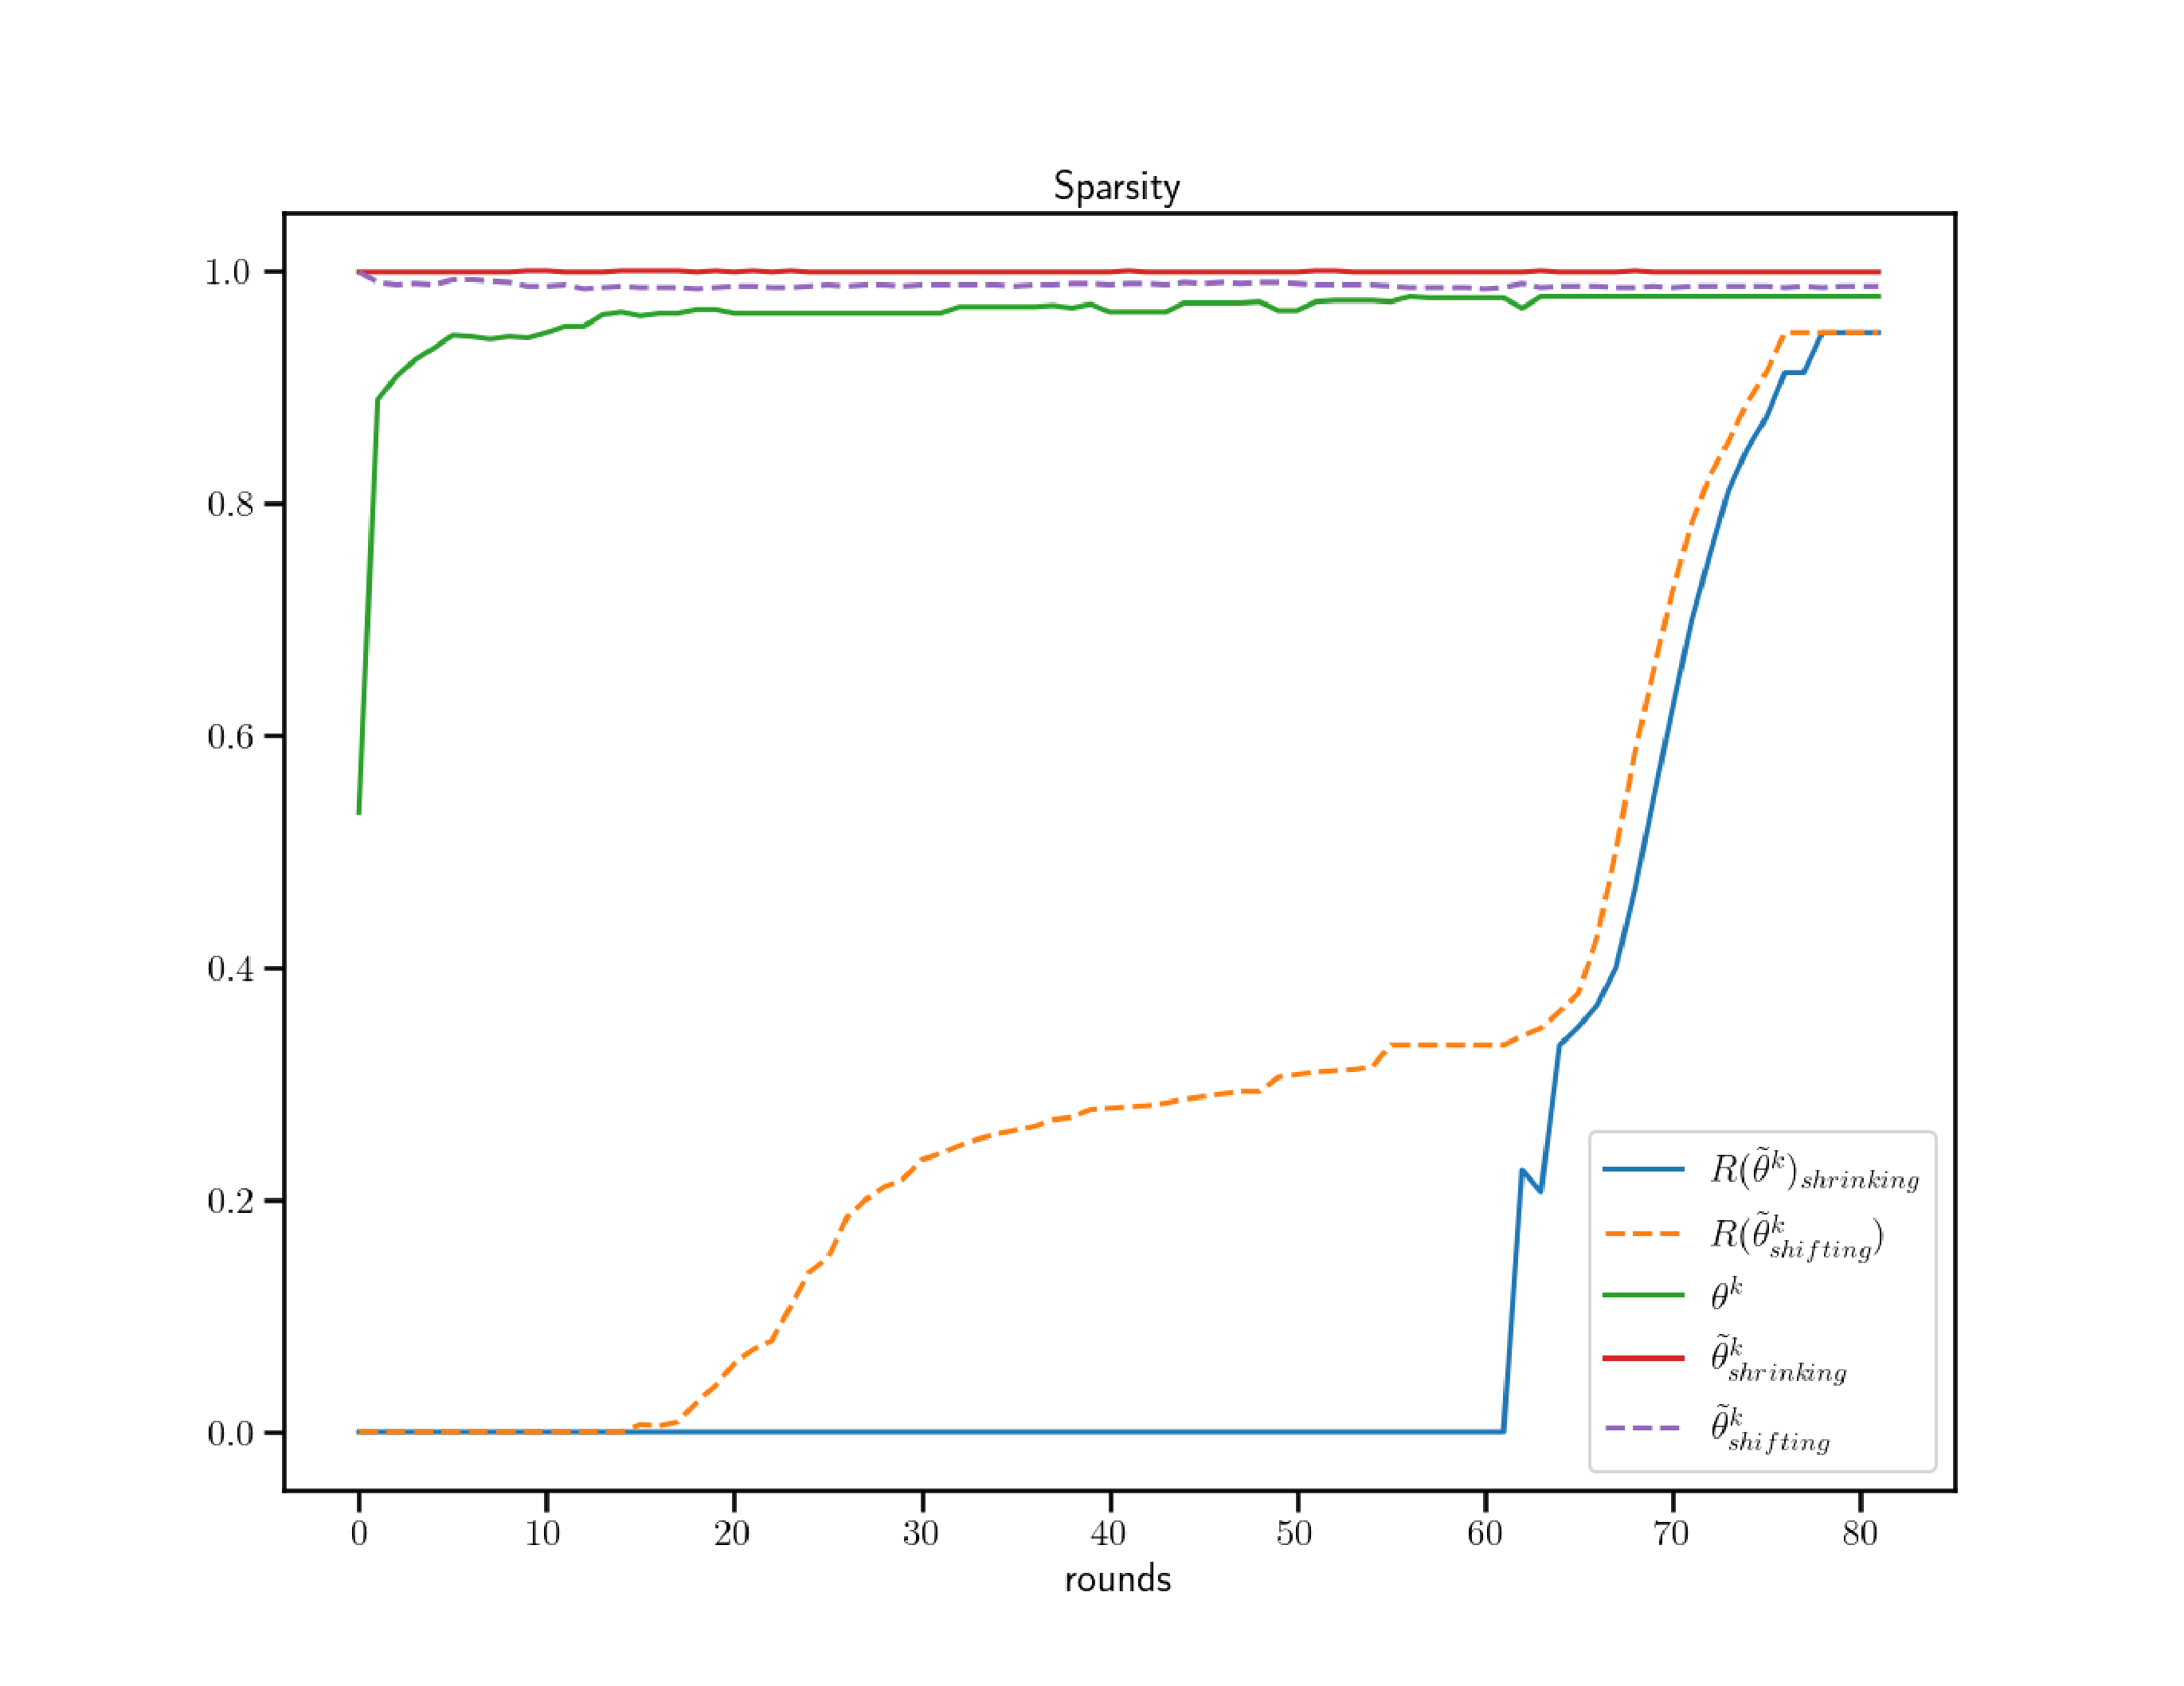
\includegraphics[width=0.4\hsize]{pic/sparse_proj}
	\caption{Screening ratio of different projection method}
	\end{center}	
	\end{figure}

\subsection{Divide Method}
We compared the screening ratio with three different method, including our Divide method, Dynamic Sasvi method and Gap method. 

	\begin{figure}[htbp]
	\begin{center}	
	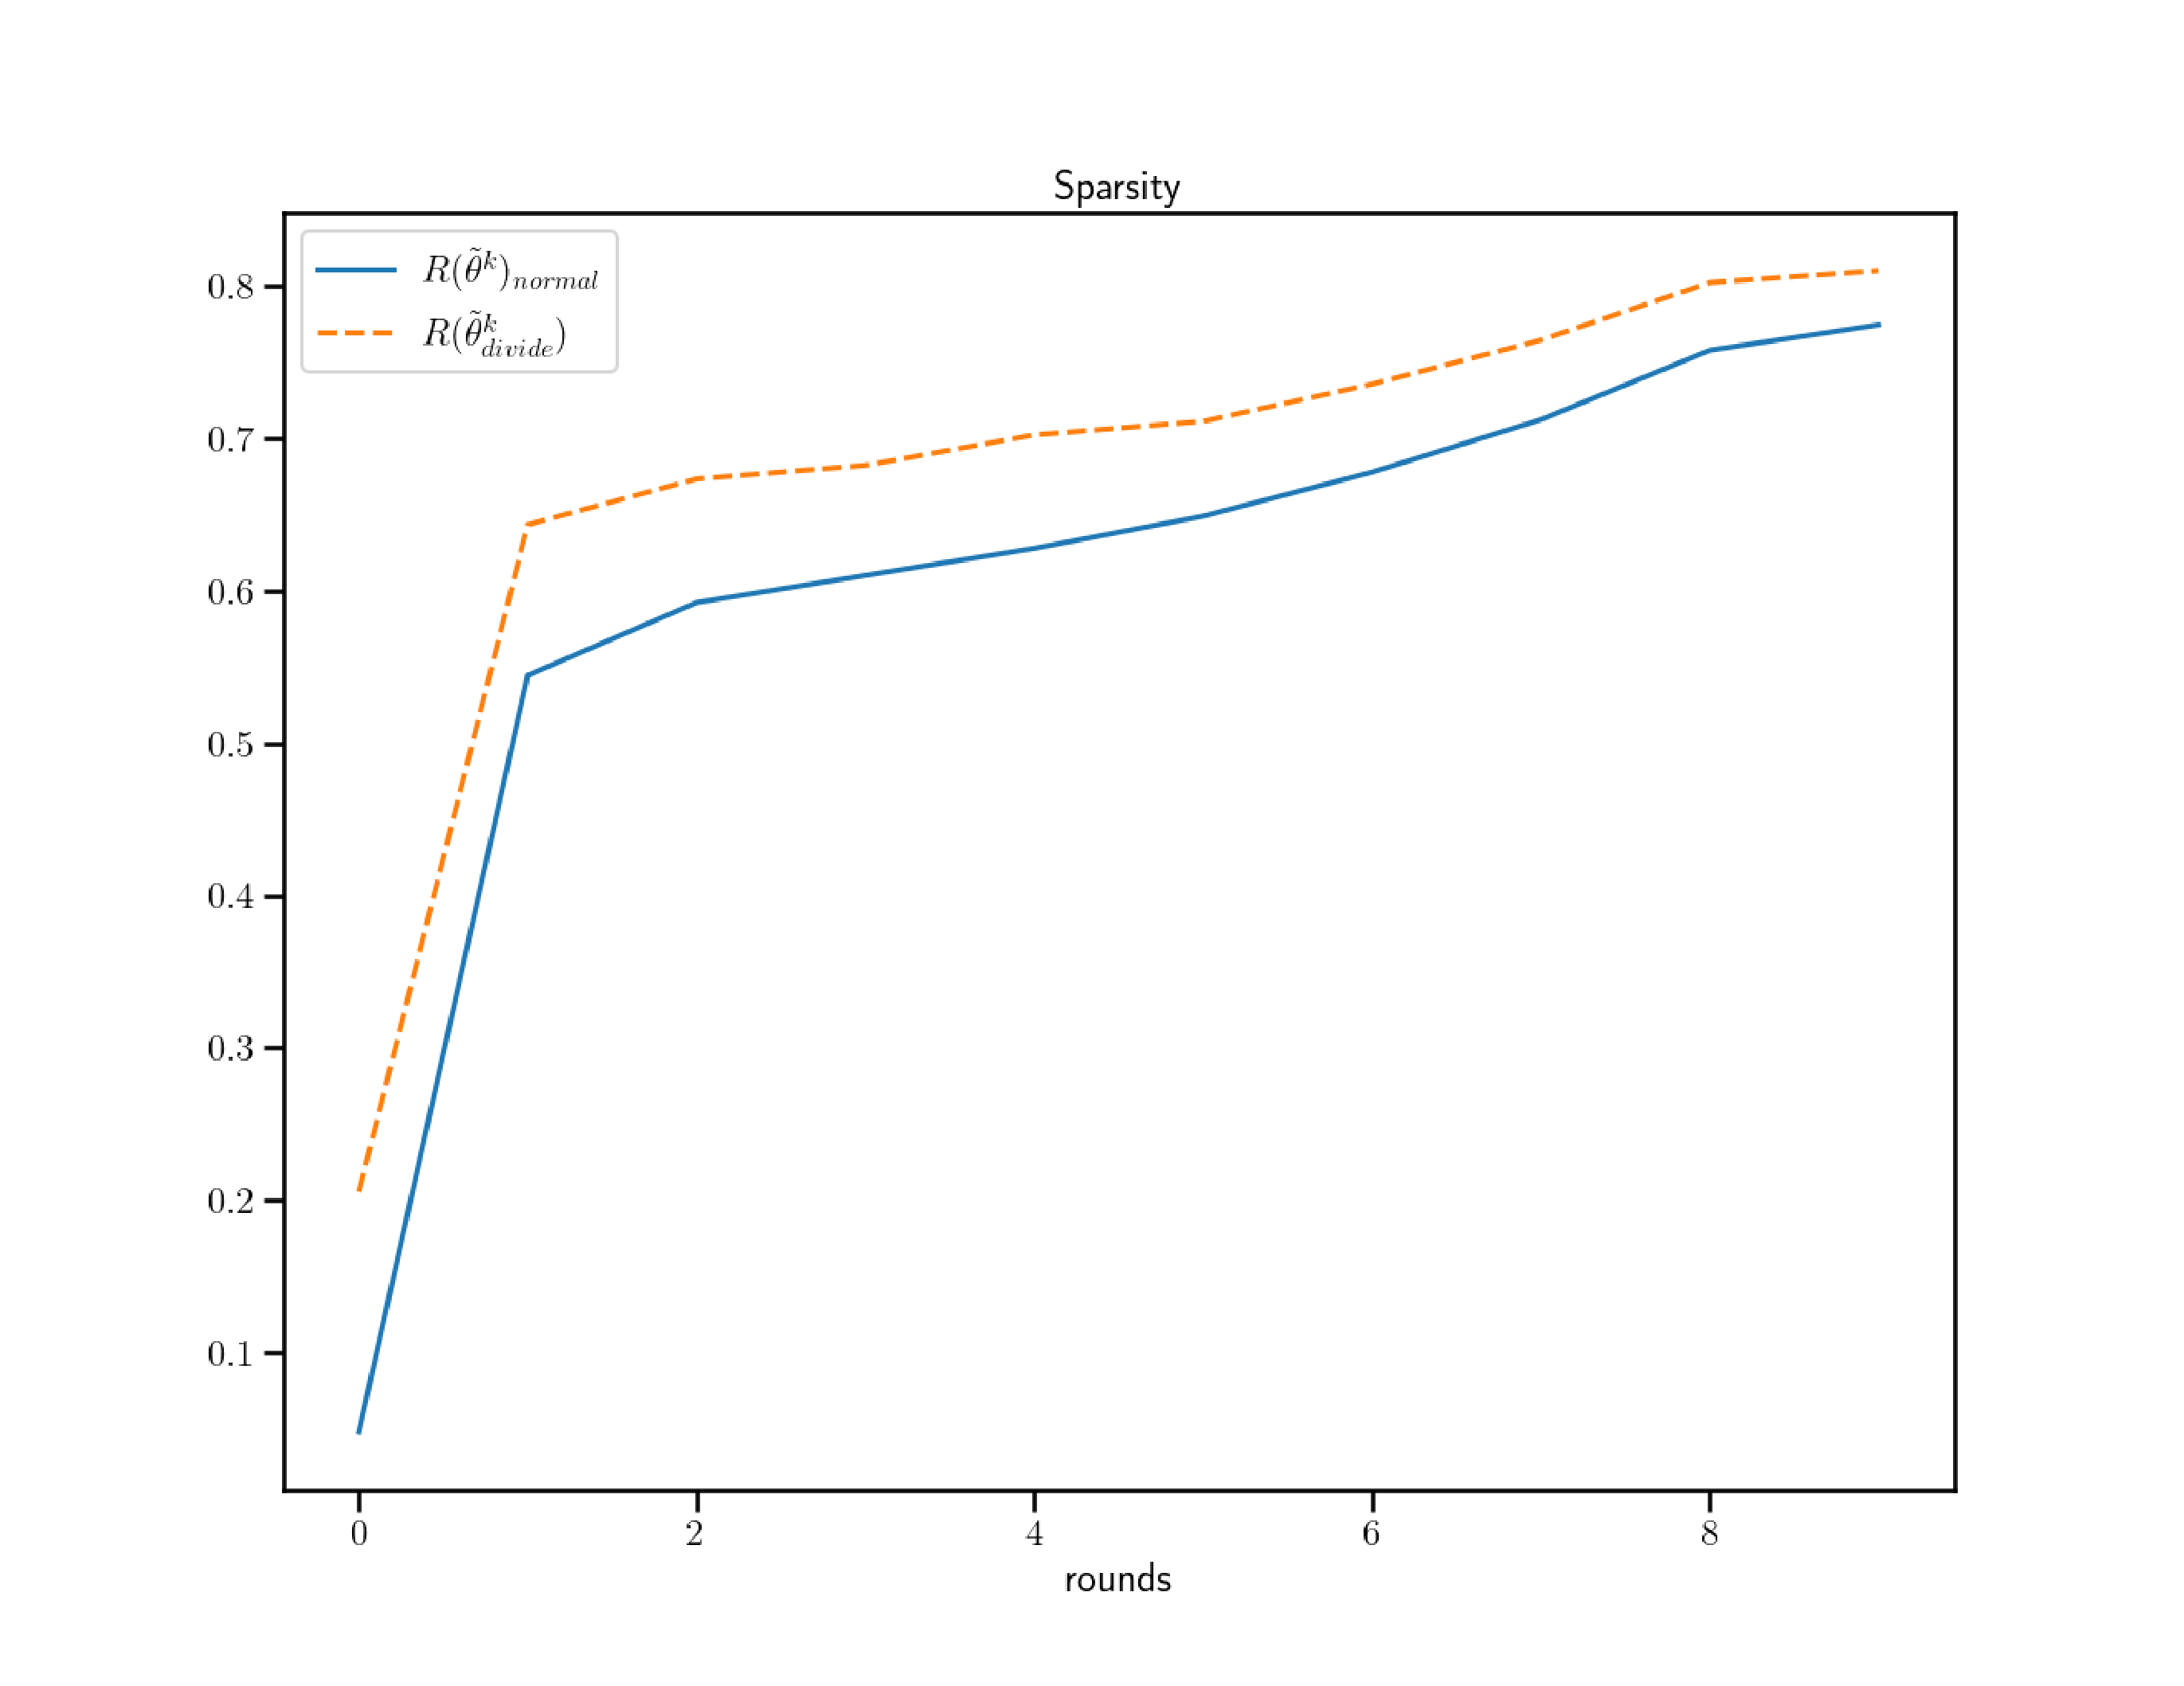
\includegraphics[width=0.4\hsize]{pic/screening_divide_ratio_long}
	\caption{Screening ratio of dividing method}
	\end{center}	
	\end{figure}

\subsection{Best divide Method}
We compared the screening ratio with three different method, including our Divide method, Dynamic Sasvi method and a random divide method.
	\begin{figure}[htbp]
	\begin{center}	
	\includegraphics[width=0.4\hsize]{pic/divide}
	\caption{Comparing of our seperation method with random seperation method}
	\end{center}	
	\end{figure}

\subsection{Speed up ratio}

We choose FISTA method, Newton method and Language method to test about the screening ratio. 
	\begin{figure}[htbp]
	\begin{center}	
	\includegraphics[width=0.4\hsize]{pic/divide}
	\caption{speed up ratio for different solver}
	\end{center}	
	\end{figure}

\section{CONCLUSION}
Our algorithm is great, we are going to apply the method onto Sinkhorn
\bibliography{ref}
\bibliographystyle{plainnat}

%%%%%%%%%%%%%%%%%%%%%%%%%%%%%%%%%%%
%%%%%% SUPPLEMENT (OPTIONAL) %%%%%%
%%%%%%%%%%%%%%%%%%%%%%%%%%%%%%%%%%%

\clearpage
\appendix

\thispagestyle{empty}


% For one-column format, uncomment the following:
\onecolumn \makesupplementtitle
% For two-column format, uncomment the following:
%\twocolumn[ \makesupplementtitle ]


\section{Entropic UOT dual}
We know that 
\begin{equation}
P(t):= \min_{t \in \mathbb{R}_{+}^{mn}} f(\X t) + g(t)
\end{equation}
the dual problem is 
\begin{equation}
D(\theta) := \max_{\theta} -f^*(-\theta) - g^*(X^{\tranT}\theta)
\end{equation}
The Entropic UOT problem is:
\begin{equation}
\label{eq:euot}
W(\alpha,\beta) := \min_{t \in \mathbb{R}_{+}^{mn}, t_i>\epsilon>0} \lambda c^{\tranT}t + D_h(\mathbf{X}t,y) + \varepsilon H(t)
\end{equation} 

$H(x) = x^{\tranT}(\ln x - 1)$, In order to screening, we introduce a smoothing threshold $t\geq \epsilon >0$ 
$$
\begin{aligned}
f(\X t) &=  D_h(\mathbf{X}t,y) \\
g(t) &= \lambda c^{\tranT} t + \varepsilon H(t)
\end{aligned}
$$

We have 
$$
\begin{aligned}
f^{*}(\theta) &= \max_t \theta^{\tranT} t -  t\ln \frac{t}{y} + t^{\tranT}\one - y^{\tranT}\one\quad (t^{*}=y \odot e^{\theta})\\
&=y^{\tranT} e^{\theta} - y^{\tranT}\one \\
g^{*}(\theta) &= \max_t \theta^{\tranT} t - \varepsilon t^{\tranT}(\ln t -1) - \lambda c^{\tranT}t \quad(t^* = \exp{\frac{\theta-\lambda c}{\varepsilon}})\\
&= \sum_{i,\theta_i\geq\lambda c_i +\varepsilon\ln \epsilon } \varepsilon \exp(\frac{\theta_i-\lambda c_i}{\varepsilon})+\sum_{i,\theta_i<\lambda c_i +\varepsilon\ln \epsilon} \epsilon(\theta_i - \varepsilon(\ln\epsilon-1)-\lambda c_i) 
\end{aligned}
$$

The dual problem is:
\begin{equation}
\label{eq:reuot}
D(\theta) := \max_{\theta} -y^{\tranT}e^{-\theta} + y^{\tranT}\one - \sum_{i,x_i^{\tranT}\theta\geq\lambda c_i +\varepsilon\ln \epsilon} \varepsilon \exp(\frac{x_i^{\tranT}\theta-\lambda c_i}{\varepsilon}) - \sum_{i,x_i^{\tranT}\theta<\lambda c_i +\varepsilon\ln \epsilon } \epsilon(x_i^{\tranT}\theta - \varepsilon(\ln\epsilon-1)-\lambda c_i)
\end{equation}

Let's have a look whether it is strongly conconcave...
$$
\begin{aligned}
\frac{\partial D}{\partial \theta} &=  y^{\tranT}e^{-\theta} -  \sum_{i,x_i^{\tranT}\theta\geq\lambda c_i +\varepsilon\ln \epsilon} x_i\exp(\frac{x_i^{\tranT}\theta-\lambda c_i}{\varepsilon}) -\sum_{i,x_i^{\tranT}\theta<\lambda c_i +\varepsilon\ln \epsilon} \epsilon x_i
\end{aligned}
$$

$$
\begin{aligned}
\frac{\partial^{2} D}{\partial \theta^{2}} &=  -\operatorname{Diag}(y^{\tranT}e^{-\theta}) -  \sum_{i,x_i^{\tranT}\theta\geq\lambda c_i +\varepsilon\ln \epsilon} \frac{x_i x_i^{\tranT}}{\varepsilon}\exp(\frac{x_i^{\tranT}\theta-\lambda c_i}{\varepsilon})
\end{aligned}
$$
L is

$$
\begin{aligned}
L(t,v,\eta,u,m) &= \min_{t,v} \max_{\eta>0,u,m} \lambda c^{\tranT}t + D_h(y,v) + \varepsilon H(t) + \eta ^{\tranT} (-t) +u^{\tranT}(v-\X t) + m( t^{\tranT}\one - a)\\
&= \max_{\eta>0,u,m} -ma + \min_{t,v}  \lambda c^{\tranT}t + D_h(y,v) + \varepsilon H(t) + \eta ^{\tranT} (-t) +u^{\tranT}(v-\X t) + m t^{\tranT}\one 
\end{aligned}
$$

\begin{equation}
\frac{\partial L}{\partial v} = 
\end{equation}

\begin{equation}
W(\alpha,\beta) := \min_{t \in \mathbb{R}_{+}^{mn}} f(\X t) + g(t)
\end{equation}
We have 
$$
f(Xt) = D_h(y,\X t) 
$$

$$
g(t) = \lambda c^{\tranT}t +  \varepsilon (t +\eta_2) \ln (t+\eta_2)
$$

$$
\begin{aligned}
g^*(\theta) &= \max_{t} \theta^{\tranT} t - g(x)\\
\frac{\partial g^*}{\partial t} &= \theta - \lambda c - \varepsilon(\ln (t+\eta_2)+1) \\
t^* &= \exp (\frac{\theta - \lambda c}{\varepsilon}-1) - \eta_2\\
g^*(\theta) &= (\lambda c-\theta)\eta_2 + \varepsilon \exp(\frac{\lambda c-\theta}{\varepsilon}-1)
\mathbf{s.t.} 
\end{aligned}
$$

\section{FORMATTING INSTRUCTIONS FOR THE SUPPLEMENTARY MATERIAL}

Your supplementary material should go here. It may be in one-column or two-column format. To display the supplementary material in two-column format, comment out the line
\begin{verbatim}
\onecolumn \makesupplementtitle
\end{verbatim}
and uncomment the following line:
\begin{verbatim}
\twocolumn[ \makesupplementtitle ]
\end{verbatim}

Please submit your paper (including the supplementary material) as a single PDF file. Besides the PDF file, you may submit a single file of additional non-textual supplementary material, which should be a ZIP file containing, e.g., code.

If you require to upload any video as part of the supplementary material of your camera-ready submission, do not submit it in the ZIP file. Instead, please send us via email the URL containing the video location.

Note that reviewers are under no obligation to examine your supplementary material.

\section{MISSING PROOFS}

The supplementary materials may contain detailed proofs of the results that are missing in the main paper.

\subsection{Proof of Lemma 3}

\textit{In this section, we present the detailed proof of Lemma 3 and then [ ... ]}

\section{ADDITIONAL EXPERIMENTS}

If you have additional experimental results, you may include them in the supplementary materials.

\subsection{The Effect of Regularization Parameter}

\textit{Our algorithm depends on the regularization parameter $\lambda$. Here we illustrate the effect of this parameter on the performance of our algorithm [ ... ]}

\begin{equation}
\begin{split} 
\frac{\partial L}{\partial \eta} &= \frac{1-\mu a_{I_1} - \nu b_{I_1}}{2\eta^2} +  \frac{1-\mu a_{I_2} - \nu b_ {I_2}}{2\eta^2} + ( {\vq^{*}}^{\tranT}\vq^{*} -r^2) + 2\eta\frac{\partial \vq^{*}}{\partial \eta}\vq^{*} +\mu a \frac{\partial \vq^{*}}{\partial \eta} + \nu b \frac{\partial \vq^{*}}{\partial \eta}\\
\frac{\partial L}{\partial \mu} &= \frac{a_{I_1} + a_{I_2}}{2\eta} + 2 \eta \vq^{*}\frac{\partial \vq^{*}}{\partial \mu} +( a^{\tranT}\vq^{*} - e_a ) + \mu a \frac{\partial \vq^{*}}{\partial \mu} + \nu b \frac{\partial \vq^{*}}{\partial \mu} \\
\frac{\partial L}{\partial \nu} &= \frac{b_{I_1} + b_{I_2}}{2\eta} + 2 \eta \vq^{*}\frac{\partial \vq^{*}}{\partial \nu} +( b^{\tranT}\vq^{*} - e_b ) + \nu b \frac{\partial \vq^{*}}{\partial \nu} + \mu a \frac{\partial \vq^{*}}{\partial \nu} 
 \end{split}
\end{equation}


\end{document}

